
\chapter{Fundamentos Teóricos}

En esta sección vamos a introducir cuales serían los conceptos teóricos más importantes que conviene tener presentes para la correcta comprensión del trabajo y sus resultados. Para ello se ha recurrido al conocimiento adquirido en asignaturas como \textbf{Visión por Computador}, \textbf{Aprendizaje Automático} así como diversos artículos que se citarán dónde sea conveniente.

\section{Aprendizaje Automático}
    \noindent Actualmente la \textbf{Inteligencia Artificial} (IA) es una rama de la informática muy popular y de gran importancia que pretende dotar a los ordenadores de una manera de razonar o solucionar problemas inteligente. En este contexto, la IA ha explorado diversos métodos para conseguir este propósito como son el estudio de Metaheurísticas, la Ingeniería del Conocimiento y más recientemente el conocido \textbf{Aprendizaje Automático} (AA). 
    
    \medskip

    \noindent Los métodos que empleamos en este trabajo pretenecen a la rama del AA, y por lo tanto es importante comenzar definiendo qué es este concepto. Para ello, disponemos de diversas definiciones proporcionadas por distintos autores: 

    \medskip

    \noindent La primera y más clásica nos la proporciona Arthur Samuel en 1959, en la cual define el AA como \textbf{el campo de estudio que da a los ordenadores la capacidad de aprender sin ser programados explícitamente}. Esta definición es muy general, pero nos permite hacernos una idea de lo que pretende conseguir este campo de estudio, que es dotar a los ordenadores de la capacidad de \entrecomillado{aprender}, generalmente a partir de una base de datos, con la idea de poder usar este conocimiento adquirido durante el aprendizaje para resolver casos nuevos del problema que la máquina no conozca previamente.
    
    \medskip

    \noindent Una definición un poco más reciente de Tom Mitchell (1998) nos dice que: \textbf{Un programa de ordenador se dice que aprende de la experiencia E respecto de alguna tarea T y alguna medida de rendimiento P, si su rendimiento en T, medido por P, mejora con la experiencia E}. Esta segunda definición nos permite identificar los elementos necesarios para poder resolver un problema mediante técnicas de AA. Así, en primer lugar necesitamos una tarea (T) que queremos resolver con ayuda de un ordenador, una experiencia (E) en esa tarea, que generalmente es una base de datos asociada al problema, y una medida de rendimiento (P) que generalmente se asocia con una función objetivo que se pretende minimizar/maximizar.

    \medskip

    \noindent Tradicionalmente, los algoritmos de AA se dividen en dos conjuntos:

    \begin{itemize}
        \item Aprendizaje Supervisado.
        \item Aprendizaje no Supervisado.
    \end{itemize}

    \medskip 
    
    \noindent No obstante, han aparecido otras técnicas más recientes como el Aprendizaje por Refuezo que son muy interesantes y usadas actualmente, pero no vamos a profindizar en ellas pues no son necesarias para el trabajo que nos ocupa.

    \subsection{Aprendizaje Supervisado}
        \noindent Los algoritmos de AA que se emplean en este conjunto se caracterizan porque disponen de una base de datos \textbf{etiquetados} de manera que para cada dato $x$ conocemos su etiqueta asociada $y$, y nuestro objetivo sería tratar de conocer la función $f$ que los relaciona, de manera que $f(x)=y$.

        \medskip

        \noindent Dentro de este grupo podemos encontrar problemas de \textbf{regresión} y de \textbf{clasificación}.

        \subsubsection{Regresión} \label{section::Regresion}
            \noindent En los problemas de regresión se pretende obtener la función $f$ que asocia correctamente a cada dato su etiqueta: 
            \begin{equation}
                f(x)=y \; \; con \; \; x\in \mathbb{R}^m \; \; y \in \mathbb{R}^n
            \end{equation}
            
            \noindent Generalmente, obtener la función $f$ exacta es complicado, por lo que se pretende aproximar mediante una función $f'$ que elegimos y que entrenaremos a partir de los datos etiquetados que se nos proporcionan. Volviendo a la definición de Tom Mitchell, en este tipo de problemas tendríamos que 
            
            \begin{itemize}
                \item T= regresión (aproximar $f$)
                \item E= El conjunto de datos $X$ etiquetados que se proporcionan para entrenar el modelo $f'$.
                \item P= función de coste asociada (generalmente se emplea el error cuadrático medio) que nos mide lo \entrecomillado{bien} que nuestra función $f'$ aproxima a $f$.
            \end{itemize}
            
            \medskip 

            \noindent Por ejemplo el si intentamos predecir $f$ mediante un modelo lineal: 

            \begin{equation}
                f'(x)= w^T x \; \; x,w \in \mathbb{R}^m
            \end{equation}

            \noindent Disponemos de un conjunto de $N$ datos 
            
            \begin{equation}
                X= \lbrace x_1, x_2 , \ldots , x_N \rbrace \; \; x_i \in \mathbb{R}^m
            \end{equation}

            \noindent Además de un conjunto de etiquetas

            \begin{equation}
                Y= \lbrace y_1, y_2 , \ldots , y_N \rbrace \; \; y_i \in \mathbb{R}^n
            \end{equation}

            \noindent Y usamos como medida de error el error cuadrático medio: 

            \begin{equation}
               J(\alpha)= \frac{1}{N} \sum_{i=1}^{N}(f'(x_i) - f(x_i))^2 = \frac{1}{N} \sum_{i=1}^{N}(y_i' - y_i)^2
            \end{equation}

            \noindent Dónde $y_i'$ es la etiqueta predicha por $f'$ para $x_i$.

            \medskip

            \noindent Nuestro objetivo sería encontrar el vector de pesos $w$ que minimice la función de coste $J$ y para ello utilizamos los datos de entrenamiento $X$.
            
        \subsubsection{clasificación}
            \noindent Por otro lado tenemos los problemas de clasificación, en los datos se encuentran agrupados en clases y se pretende clasificar cada dato de entrada en la clase correcta. Los casos más sencillos de este problema son los de \textbf{clasificación binaria}, y en ellos se pretende agrupar los datos en dos posibles clases que suelen codificarse como $0$ y $1$.

    \subsection{Aprendizaje no Supervisado}
            \noindent El aprendizaje no supervisado se caracteriza porque los datos que se proporcionan no están etiquetados, y no se busca una salida concreta, sino que se pretende analizar las características de nuestro conjunto de datos. 

            Así, por ejemplo, tareas que pueden resolverse con esta técnica pueden ser la agrupación de clientes de cierta compañía en distintas clases según sus características.
            
    \subsection{Nuestro Problema}
        \noindent En nuestro problema, los frameworks de los que disponemos resuelven problemas de aprendizaje supervisado y no supervisado. 
        
        \medskip
        
        \noindent Por ejemplo vamos a intentar predecir los landmarks cefalométricos para una cierta imagen de entrada, lo que nos llevaría a un problema típico de aprendizaje supervisado en el que pretendemos a partir de la imagen de entrada conocer la función que nos proporciona la salida correcta (la imagen con los landmarks marcados correctametne).

        \medskip

        \noindent Por otro lado, uno de nuestros frameworks tiene una etapa de entrenamiento previa al problema de los landmarks en la cual mediante conjuntos de datos de imágenes sin etiquetar de rostros humanos, se pretende reconstruir imágenes preservando al máximo posible la estructura de la cara. Esto, como podemos ver, es un problema típico de aprendizaje no supervisado, porque no se busca obtener una etiqueta para cada imagen, sino analizar la estructura de los distintos elementos de los datos de entrada para ser capaces de reconstruirlos preservando su estructura.

    \subsection{Gradiente Descendente}
        \noindent En esta sección hemos hablado de qué es el AA y cómo se formalizan sus problemas para poder resolverlos. Y en concreto hemos formalizado cómo se resuelven los problemas de regresión en los que queríamos aproximar una función desconocida $f$ a partir de una aproximación $f'$ y en base a una función de coste. Sin embargo, no hemos hablado de ningún algoritmo que se use en la minimización de dicha función de coste. Es por ello que vamos a explicar el principal algoritmo que se utiliza para esta tarea, el \textbf{Gradiente Descendente}. 

        \medskip

        \noindent El Gradiente descendente es un algoritmo clásico que persigue la idea intuitiva de que el gradiente de una función siempre \entrecomillado{apunta} hacia el máximo de esta, por lo que seguir la dirección contraria a este nos llevará al mínimo de la función. Más formalmente, si recuperamos la notación del apartado \autoref{section::Regresion} tendríamos: 

        \medskip
        
        \noindent La función objetivo es: 
        \begin{equation}
            f(x)=y \; \; x \in \mathbb{R}^m \; \; y \in \mathbb{R}^n
        \end{equation}

        \noindent La función con la que vamos a intentar aproximar la función objetivo es:
        \begin{equation}
            f'(x,w)=y \; \; x \in \mathbb{R}^m \; \; y \in \mathbb{R}^n \; \; w \in \mathbb{R}^d 
        \end{equation}

        \noindent La función de coste sería $J(w)$ que de alguna manera mide la distancia entre $f$ y $f'$ y que para poder aplicar el método debe ser derivable. Algunas funciones de coste usuales son: 

        \begin{itemize}
            \item La función \textbf{L2} (también conocida como error cuadrático medio): 
            \begin{equation}
                J(w)=\frac{1}{N} \sum_{i=1}^N(f(x_i,w)-f'(x_i))^2
            \end{equation}
            \item La función \textbf{L1} (también conocida como error absoluto medio): 
            \begin{equation}
                J(w)=\frac{1}{N} \sum_{i=1}^N \left|f(x_i,w)-f'(x_i)\right|
            \end{equation}
        \end{itemize}

        \noindent Una vez hemos formalizado el problema, el algoritmo \textbf{Gradiente Descendente} consiste en: 

        \begin{itemize}
            \item Se inicializa el vector de pesos $w$.
            \item En cada paso $i$ del entrenamiento, el vector de pesos del siguiente paso $i+1$ se calcula de acuerdo a la siguiente relación: 
            \begin{equation}
                w_{i+1}=w_i-\eta \nabla J(w)
            \end{equation}
            \noindent Dónde $\eta$ es un factor conocido como \textbf{learning rate}(lr) que mide el \entrecomillado{tamaño} del paso que en cada iteración damos en búsqueda del mínimo. 
        \end{itemize}

        \noindent Idealmente, con este método se encuentra un mínimo global de la función de coste en el caso en que esta sea convexa. En caso de no serlo podría caer en un mínimo local en su lugar. 

        \medskip

        \noindent Por otro lado, cabe destacar la importancia de una buena elección del \textbf{learning rate}, pues si este es demasiado pequeño puede ocasionar una lenta convergencia al mínimo, y por lo tanto que se realice un gran número de iteraciones, y en cambio un valor excesivamente grande de este puede impedir la convergencia,pues los saltos serían tan grandes en la dirección del mínimo local o global que podría llegar a \entrecomillado{saltar} por encima de este siempre. Por lo tanto una técnica habitual aunque costosa de este algoritmo consiste en usar un learning rate adaptativo, que sea mayor en las primeras iteraciones y que vaya disminuyendo conforme se incremente el número de iteraciones (pues se entiende que se estará cerca del mínimo).

        \subsubsection{Gradiente Descendente Estocástico}

            \noindent El algoritmo descrito anteriormente tiene el problema de ser costoso computacionalmete, debido a que en cada iteración se debe calcular la función de coste para todos los ejemplos del conjunto de entrenamiento $X$. Es por ello que suele emplearse en su lugar una versión modificada y que sigue dando buenos resultados que consiste en actualizar los pesos en base a unos pocos ejemplos del conjunto de entrenamiento $X$ que se conoce como \entrecomillado{minibatch}.




\section{Visión por Computador}
    \noindent La \textbf{Visión por computador} es un área de conocimiento en el que se unen diversas disciplinas como la IA o el AA para un propósito común, que es el procesado de imágenes por medio de un ordenador con la finalidad de que la máquina pueda llegar a extraer información relativa a estas del mismo modo en que lo haría un ser humano \cite{rosenfeld1988computer}. 

    \medskip
    
    \noindent Problemas clásicos de la visión por computador son el reconocimiento de objetos o personas en imágenes, la segmentación o la clasificación. Así pues, podemos ver la relación directa que hay entre nuestro objetivo y esta disciplina, pues los frameworks que usaremos tendrán por objetivo extraer información de imágenes de rostros de personas para posteriormente tratar de identificar en ellos con el mayor grado de decisión posible una serie de landmarks cefalométricos que el sistema ha aprendido a base de unos ejemplos etiquetados (AA).

    \medskip

    \noindent Finalmente, en los últimos años esta rama ha experimentado un fuerte crecimiento e importancia en la comunidad científica debido al actual desarrollo del \textbf{Deep Learning} y las \textbf{redes convolucionales profundas} que explicaremos en detalle en la siguiente sección. Estas nuevas herramientas han permitido crear programas que obtienen un gran rendimiento en el tratamiento de imágenes. Ejemplo de ello son los dos frameworks que vamos a comparar en este trabajo.

\section{Deep Learning}
    Como ya se ha mencionado anteriormente, la IA se encuentra muy desarrollada actualmente y es capaz de resolver problemas que tradicionalmente eran muy complicados para ser resueltos por un humano, pero que se ha demostrado que no son tan complicados para una máquina. Sin embargo, e irónicamente, algunas de las tareas más fáciles para los seres humanos como son el reconocimiento del habla o la identificación de objetos en imágenes han suponen un verdadero reto para un odernador, y o ha sido hasta los últimos años con el nacimiento del \textbf{Deep Learning} que se han empezado a obtener resultados satisfactorios en este campo.
    
    Por lo tanto, los algoritmos del Deep Learning se caracterizan por resolver estos problemas a partir de representaciones del mismo que se expresan en terminos de otras más simples. De esta manera se pueden construir conceptos difíciles a partir de otros más sencillos. Este grafo puede ser tan profundo como se necesite, por ello se le conoce como Deep Learning.

    \subsection{Redes Neuronales} \label{sub:redes_neuronales}
        La arquitectura básica de los modelos de Deep Learning viene descrita por la arquitectura de una \textbf{red neuronal}. Es por ello que vamos a profundizar un poco en esta estructura y para ello vamos a partir de un ejemplo clásico como es el \textbf{Perceptrón multicapa}(MLP). Para esta sección vamos a seguir el capítulo 6 de \cite{Goodfellow-et-al-2016}.

        \medskip

        \noindent Las redes neuronales tienen por objetivo aproximar una función desconocida $f(x)=y$ que asocia a cada entrada $x$ una salida $y$ a partir de una función $f'(x;W)= \widehat{y}$ (dónde $\widehat{y}$ es la etiqueta predicha para la entrada $x$) que depende de unos parámetros $W$, de manera que el objetivo es aprender los valores de $W$ que mejor aproximan la función objetivo $f$.

        \medskip

        \noindent Se denominan algoritmos \textbf{feedforward} porque la información fluye desde la entrada $x$ a través de los cálculos intermedios que definen $f'$ hasta finalmente dar una salida $y$.

        \medskip

        \noindent Finalmente a estos algoritmos se les denomina \textbf{redes} porque generalmente se representan como una composición de distintas funciones en cadena de manera que se van aplicando sucesivamente sobre la entrada $x$ hasta la salida $\widehat{y}$. 

        \begin{figure}[!h]
            \centering
            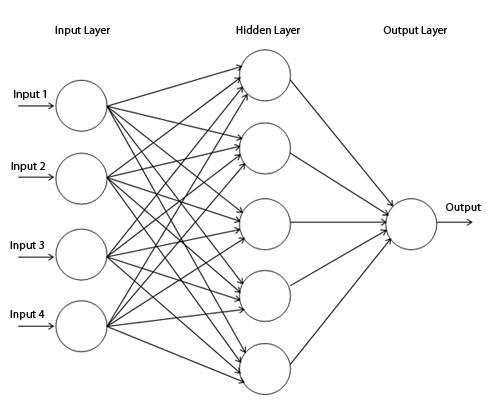
\includegraphics[width=0.5\textwidth]{img/single_hidden_layer.jpg}
            \caption{Red neuronal con una capa oculta. Formalmente podría describirse como $f'(x)=(f_3(f_2(f_1(x))))$, dónde $f_1$ hace referencia a la capa de entrada a la red, $f_2$ a la capa oculta y $f_3$ a la capa de salida.}
            \label{fig:red_neuronal_capa_oculta}
          \end{figure}

        \noindent La \textbf{profundidad} de la red vendría dada por la cantidad de \textbf{capas ocultas} que esta tiene. En los algoritmos de Deep Learning veremos un gran número de capas ocultas, de ahí el nombre. 

        \medskip

        \noindent Por otro lado, cada capa contiene un número determinado de \textbf{neuronas}, que se relacionan con las de la capa siguiente y las de la capa anterior mediante combinaciones lineales generalmente. Sin embargo, estas combinaciones lineales no son suficientes para que la red pueda aproximar funciones objetivo $f$ que sean no-lineales, para ello se emplean las llamadas \textbf{funciones de activación}. Se tratan de un conjunto de funciones no-lineales entre las que destacan las siguientes \cite{sharma2017activation}: 

        \begin{itemize}
            \item \textbf{Función Sigmoide}. Transforma los valores de entrada a un valor entre $0$ y $1$.
            \begin{equation}
                Sigmoide(x)=\frac{1}{e^{-x}}
            \end{equation}
            \item \textbf{Función Tangente Hiperbólica}. Es similar a la función sigmoide, pero es simétrica respecto al origen. 
            \begin{equation}
                tanh(x)=\frac{e^x - e^{-x}}{e^x + e^{-x}} 
            \end{equation}
            \item \textbf{Función ReLU}. Es una de las más usadas en redes neuronales por ser de las más eficientes, ya que permite que no se activen todas las neuronas a la vez, ya que en aquellas cuya salida tras la combinación lineal con los pesos de la capa correspondiente sea 0 no serán activadas.
            \begin{equation}
                ReLU(x)=\max(0,x)
            \end{equation}

            \noindent Existe el problema de que en algunos casos, el gradiente de la función sea $0$ debido a que los pesos no se actualicen durante el proceso que explicaremos más adelante de \textbf{back-propagation}.

            \item \textbf{Función Leaky ReLU}. Es una versión mejorada de la función anterior, ya que para los casos en los que la función anterior valía $0$, ahora se expresan como una componente lineal de la entrada $x$ muy pequeña, de esta manera se resuelve el problema de que el gradiente de la función sea $0$. 
            \begin{equation}
                LeakyReLU(x)=\left\{ \begin{array}{lcc}
                    x &   si  & x \leq 0 \\
                    \\ ax &  si & 0 < x \\
                    \end{array}
                \right.
            \end{equation}

            \noindent Dónde $a$ es un valor muy próximo a $0$.
            \item \textbf{Función SoftMax}. Es una combinación de múltiples funciones sigmoide. Mientras que la función Sigmoide se usa en problemas de clasificación binaria, la función SoftMax permite que se pueda realizar clasificación multiclase, ya que transforma un vector de entrada K-dimensional de valores reales en un vector K-dimensional de elementos entre $0$ y $1$, de manera que la componente más próxima a $1$ podría entenderse como la clase a la que pertenecería el elemento en un problema de clasificación multiclase.
            
            \begin{equation}
                \sigma(x)_j= \frac{e^{z_j}}{\sum_{k=1}^{K}e^{z_k}} \; \; j=1, \ldots, K
            \end{equation}
        \end{itemize}

        \noindent No existe una manera de elegir la mejor función para cada caso, pero de forma experimental se ha podido comprobar que la función ReLU en general da buenos resultados y si hubiera demasiadas neuronas muertas en la red podría cambiarse por la Leaky ReLU.

        \medskip

        \noindent De esta manera, en la capa $i$ de la red, la función $f_i$ suele tener la siguiente expresión: 

        \begin{equation}
            f_i(x)=\gamma(w_i^T x)
        \end{equation}

        \noindent Dónde $\gamma$ representa una función cualquiera del conjunto de funciones de activación que hemos descrito antes y $w_i$ el vector de pesos correspondiente a la capa $i$ de la red.
    
    \subsection{Back Propagation}
        Todas las funciones de las capas intermedias de la red son derivables, por lo que se podría calcular de forma explícita su expresión en cada caso, lo que ocurre es que este proceso es costoso computacionalmete. En lugar de esto se aplica la técnica de \textbf{Back-propagation}.

        \medskip

        \noindent Para entender este proceso correctamente se debe introducir primero el concepto de \textbf{Grafo Computacional}, que no es otra cosa que representar una función mediante un grafo. Como por ejemplo \autoref{fig:GrafoComputacional}.

        \begin{figure}[!h]
            \centering
            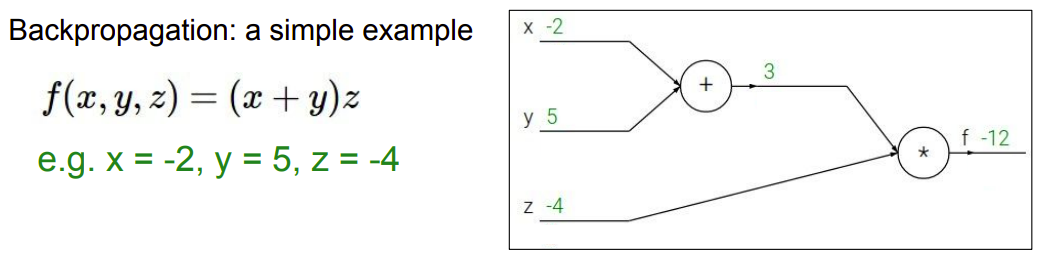
\includegraphics[width=0.8\textwidth]{img/GrafoComputacional.png}
            \caption{Ejemplo de Grafo computacional junto con la salida para una entrada concreta $x=-2$,$y=5$, $z=-4$. La imagen ha sido extraida del curso \cite{StanfordCourse}.}
            \label{fig:GrafoComputacional}
        \end{figure}

        \medskip

        \noindent La idea del algoritmo de Back-propagation es ir calculando la derivada en cada nodo del grafo computacional mediante la aplicación de la regla de la cadena, de manera que si $f(x,y,z)=g(x,y)h(z)$ si quisiéramos calcular $\frac{\partial f}{\partial x}$ aplicando la regla de la cadena tendríamos que: 

        \begin{equation}
            \frac{\partial f}{\partial x}= \frac{\partial f}{\partial g} \frac{\partial g}{\partial x}
        \end{equation}

        
        Podemos entender mejor el proceso resolviendo el ejemplo \autoref{fig:GrafoComputacional}: 

        \begin{figure}[!h]
            \centering
            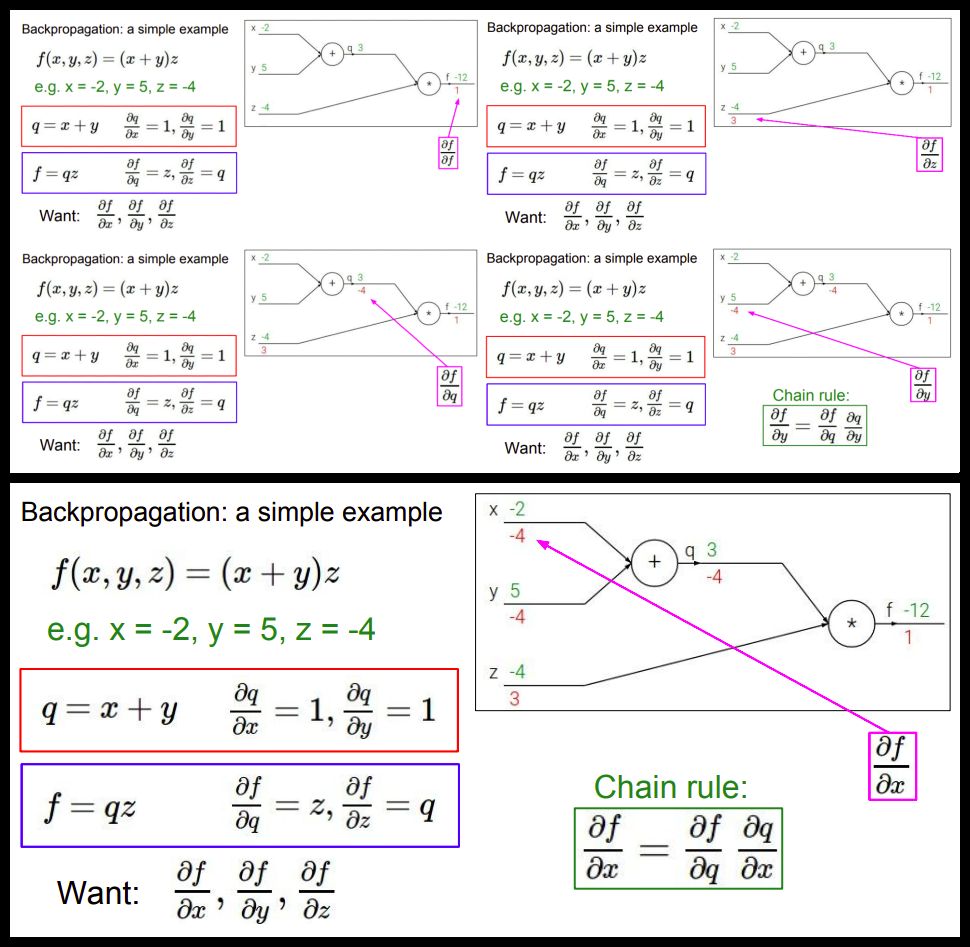
\includegraphics[width=0.8\textwidth]{img/BP_ejemplo.png}
            \caption{Como podemos ver en la imagen superior, en primer lugar se renombra la salida de la operación $x+y$ por $q$, de manera que $f=qz$. Tras esto se empiezan a calcular las derivadas parciales correspondientes desde el final hacia la entrada, aplicando cuando sea necesario la regla de la cadena hasta obtener la derivada de cada nodo en la imagen de abajo. Las imágenes han sido extraidas de \cite{StanfordCourse}}
            \label{fig:Ejemplo BP}
        \end{figure}

        \noindent Como vemos en \autoref{fig:Ejemplo BP}, se produce un flujo desde la salida hacia la entrada en la que se van calculando los gradientes para cada parámetro. Una vez calculado el gradiente se procede a actualizar los pesos usando por ejemplo el algoritmo de \textbf{gradiente descendente}.
    
\section{Redes Neuronales Convolucionales}
    \noindent Las \textbf{Redes Neuronales Convolucionales} (CNN) son la principal herramienta del Deep Learning y están inspiradas en las redes neuronales que hemos explicado anteriormente, con la salvedad de que ahora en vez de tener como entrada un vector de $\mathbb{R}^d$ ahora pueden entrar a la red volúmenes de datos en varias dimensiones, como por ejemplo imágenes que se representan como una matriz $2$D.
    
    \medskip

    \noindent La principal motivación para la creación de estas redes es el concepto de \textbf{conectividad local}, pues cuando se trabaja con entradas de grandes dimensiones como son las imágenes, resulta impráctico conectar cada neurona con todas las de la capa anterior (como suele ocurrir en las redes neuronales clásicas que hemos visto anteriormente). Es por ello que se decide conectar cada neurona con una región local del volumen de entrada. Por lo que vamos a emplear filtros que siempre van a tener la misma profundidad que el volumen de entrada y que vamos a ir desplazando a lo largo del volumen de entrada. A continuación vamos a ver qué operación realizaremos con este filtro sobre el volumen de la imagen que ocupa para alimentar cada neurona de la siguiente capa.

    \medskip

    \noindent Se denominan \textbf{Convolucionales} debido a que la principal operación matemática que realiza en cada filtro es la convolución. La operación de convolución se realiza generalmente entre dos funciones de variable real y viene descrita por la siguiente expresión:

    \begin{equation}
        f(t)=\int g(a) h(t-a) da = (g \ast h)(t)
    \end{equation}

    \noindent Dónde $t$ generalmente representa el paso del tiempo y $x,w$ son dos funciones de variable real.

    \medskip

    \noindent Sin embargo, la expresión anterior es la definición en el caso continuo, por lo que al trabajar en un ordenador, el tiempo y las funciones que empleamos deben ser discretizado, por ello consideraremos que $t$ toma solo valores enteros.De esta forma, definimos la \textbf{convolución discreta} en una dimensión como: 

    \begin{equation}
        f(t)= (g \ast h)(t) = \sum_{a=-\infty}^\infty g(a) h(t-a)
    \end{equation}

    \medskip

    \noindent Sin embargo, en nuestro caso aplicaremos las CNN a imágenes, que se discretizan como matrices $2$D, por lo que necesitamos extender la definición anterior al caso de dos dimensiones: 

    \begin{equation}
        f(n,m)= (g \ast h)(n,m) = \sum_{j=-\infty}^\infty \sum_{i=-\infty}^\infty g(i,j) h(n-i,m-j)
    \end{equation}

    \noindent La convolución tiene las siguientes propiedades: 

    \begin{itemize}
        \item \textbf{Conmutatividad}: 
        \begin{equation}
            f \ast g = g \ast f
        \end{equation}
        \item \textbf{Asociatividad}: 
        \begin{equation}
            f \ast (g \ast h) = (f \ast g) \ast h
        \end{equation}
        \item \textbf{Distributividad}: 
        \begin{equation}
            f \ast (g + h)= (f\ast g) + (f \ast h)
        \end{equation}
    \end{itemize}

    \noindent Con esto tenemos todos los ingredientes para empezar a describir la estructura de una CNN, que generalmente se compone de tres tipos de capas: \textbf{capas convolucionales}, \textbf{capas de Pooling} y \textbf{capas totalmente conectadas}.

    \subsection{Capa Convolucional}
        \noindent Se trata de la capa esencial de una CNN y consiste en desplazar un filtro por todo el volumen de entrada realizando la operación de convolución discreta en $2$D. Como dijimos antes, la profundidad del filtro que empleamos para esto coincide con la del volumen de entrada siempre. Vamos a discutir ahora qué volumen de salida genera cada capa convolucional que viene definido por tres parámetros: \textbf{depth}, \textbf{stride} y \textbf{padding}

        \begin{itemize}
            \item El parámetro \textbf{depth} se corresponde con el número de filtros que queremos aplicar al volumen de entrada, pues se pretende que cada uno de ellos aprenda algo distinto sobre este. Como cada filtro produce un volumen $m \times n$ de profundidad $1$ conocido como \textbf{mapa de activación}, este parámetro nos genera tantos mapas de activación como indique.
            \item El parámetro \textbf{stride} indica el paso con el que vamos desplazando cada filtro sobre el volumen de entrada, así un stride de $1$ indica que el filtro se desplaza de uno en uno por los píxeles, y un stride de $2$ indicaría que se desplaza de dos en dos. Cuanto mayor sea de menores dimensiones será el mapa de activación.
            \item El parámetro \textbf{padding} indica en cuantas filas y columnas se amplía el volumen de entrada antes de aplicar los filtros. Este parámetro se utiliza para controlar la dimensión de salida de los mapas de activación pues la convolución es una operación que reduce la dimensionalidad siempre.
        \end{itemize}

        \noindent Con todo esto en mente, la relación que determina el volumen de salida de una capa convolucional para un volumen de entrada de dimensión $W \times W \times d$ y empleando filtros de dimensión $F \times F \times d$ con un padding $P$, un stride $S$ sería: 

        \begin{equation}
            Output=(W-F + 2P)/S + 1
        \end{equation}

        \medskip
        
        \noindent Generalmente la salida de cada capa convolucional supone la entrada a una función de activación como las que se describieron en \autoref{sub:redes_neuronales}. Normalmente se utiliza la función ReLU, aunque también es común el uso de Leaky ReLU.

        \begin{figure}[!h]
            \centering
            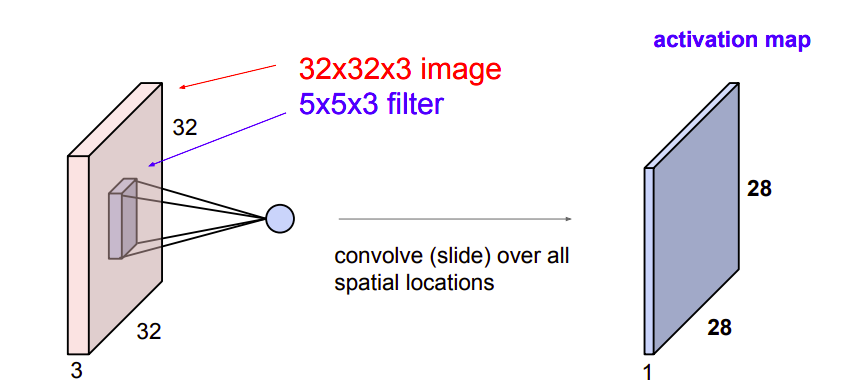
\includegraphics[width=0.8\textwidth]{img/mapa_activacion.png}
            \caption{Ejemplo de cálculo de mapa de activación en una capa convolucional para un determinado volumen de entrada. El parámetro depth nos dice la cantidad de mapas de activación generamos para el volumen de entrada, o dicho de otro modo, el número de filtros que aplicamos. La imagen ha sido extraida de \cite{StanfordCourse}}
            \label{fig:mapa_activacion}
        \end{figure}

        \begin{figure}[!h]
            \centering
            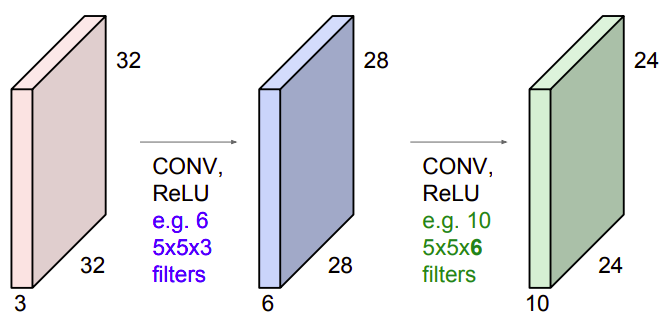
\includegraphics[width=0.8\textwidth]{img/sucesion_conv_layer.png}
            \caption{Sucesión de varias capas convolucionales + ReLU que describen la estructura básica de una CNN. Cabe destacar como la produndidad de los filtros es siemore la misma que la del volumen de entrada, de acuerdo a lo que hemos dicho anteriormente. La imagen han sido extraida de \cite{StanfordCourse}}
            \label{fig:estructura_convnet}
        \end{figure}

    \subsection{Capa de Pooling}
        \noindent En las CNN es normal instertar de vez en cuando capas de Pooling. Esta capa reduce la dimensión del volumen de entrada y actúa independientemente del volumen de la profundidad que tenga el volumen de entrada. Generalmente se emplean filtros de dimensión $2 \times 2$ con un stride de $2$ que reduce a la mitad la dimensión del volumen de entrada y mantiene la profundad.

        \medskip

        \noindent El tipo de operación que se realiza con el filtro $2 \times 2$ ha sido objeto de estudio en los últimos años, y se han probado las siguientes funciones: 

        \begin{itemize}
            \item \textbf{Max Pooling}. Consiste en tomar el máximo de los cuatro elementos que ve el filtro del volumen de entrada. 
            \item \textbf{Average Pooling}. Consiste en realzar un promedio de los elementos que ve el filtro.
        \end{itemize}

        \noindent Generalmente, el \textbf{max pooling} parece tener un mayor rendimiento en la práctica, pero esto aún es objeto de estudio.

        \begin{figure}[!h]
            \centering
            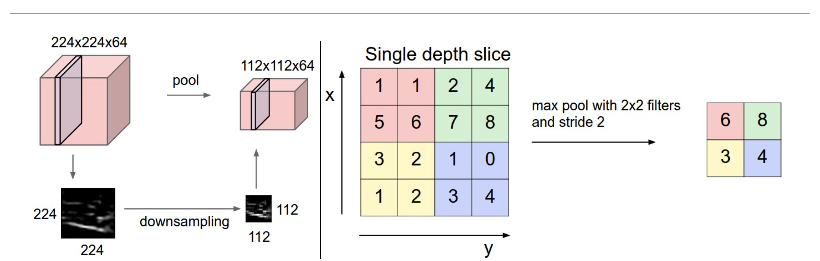
\includegraphics[width=0.8\textwidth]{img/pooling.png}
            \caption{Ejemplo de capa de pooling usando la operación del máximo. La imagen han sido extraida de \cite{StanfordCourse}}
            \label{fig:pooling}
        \end{figure}
    
    \subsection{Capa Totalmente Conectada (Fully Conected)}
        \noindent Generalmente al final de las CNN suele encontrarse una capa totalmente conectada (FC) que tiene la misma estructura que una red neuronal clásica con una o dos capas ocultas generalmente, y por lo tanto está creada para un vector de entrada de una dimensión concreta.

        \medskip

        \noindent Como hemos visto en las capas anteriores, una CNN actua de manera independiente de las dimensiones del volumen de entrada a la red salvo en las capas totalmente conectadas, es por ello que estas capas son las que normalmente determinan el volumen de entrada a la red para que esta funcione correctamente.

    \subsection{Batch Normalization}
        \noindent Actualmente, es muy común en las CNN usar \textbf{Batch Normalization} que consiste en normalizar los datos de entrada a cada capa convolucional con la intención de hacer que las operaciones convolucionales sean independientes unas de otras, es decir, que la distribución de los datos de entrada a una capa no dependa de los parámetros aprendidos por la capa anterior. Además este procedimiento ayuda a prevenir el overfitting de la red, ayudando a la regularización.

    \subsection{Optimizador Adam}
        El proceso de aprendizaje en las CNN se realiza de manera similar al caso de las redes neuronales clásicas, mediante la técnica de Back-propagation. Sin embargo el optimizador Gradiente Descendente que hemos presentado en secciones anteriores tiene un único learning rate para todos los pesos de la red y se mantiene fijo durante todo el entrenamiento. Es por ello que en su lugar generalmente se usa el optimizador Adam que permite establecer un learning rate distinto para cada parámetro y que además es adaptativo.

    \subsection{Proceso de entrenamiento de una CNN}

        \noindent Una vez aclarados todos los conceptos previos estamos en condiciones de comprender el proceso clásico de entrenamiento de una CNN en el que nos basaremos para entrenar nuestro modelo en secciones posteriores: 

        \medskip

        \noindent Generalmente se entrenan las imágenes por conjuntos denominados \textit{mini-batches}, los cuales: 

        \begin{itemize}
            \item En una primera instancia se propagan hacia adelante por toda la red calculando las activaciones y errores de salida en lo que se conoce como \textbf{forward pass}.
            \item Vamos de la salida a la entrada calculado los gradientes de cada unidad con lo que se conoce como \textbf{backward pass} aplicando el algoritmo de back-propagation.
            \item Se actualizan los pesos en base al gradiente calculado en el paso anterior y según el optimizador que se esté empleando (Adam, gradiente descendente, etc...)
        \end{itemize}

    \subsection{Evolución de las CNN}
    Una vez hemos presentado las CNN y sus principales componentes vamos a dar un breve repaso por la historia y evolución de su arquitectura \cite{EvolutionCNN}.

    \subsubsection{LeNet-5}
        \noindent La primera arquitectura conocida que forma parte de las CNN fue desarrollada por LeCun \cite{lecun1998gradient} para el reconocimiento de dígitos manuscritos, a dicha red la llamaron \textbf{LeNet-5} y fue la que sirvió de inspiración para el desarrollo de las posteriores redes.

        \begin{figure}[!h]
            \centering
            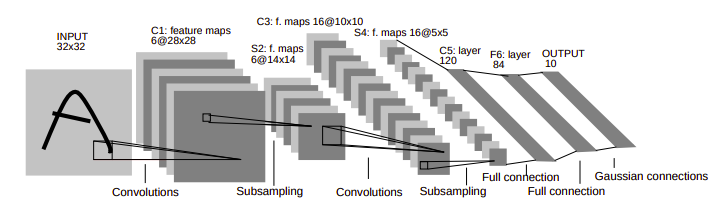
\includegraphics[width=0.8\textwidth]{img/LeNet.png}
            \caption{Arquitectura de la red LeNet. Como podemos observar tiene capas convolucionales, capas de average pooling y capas totalmente conectadas al final. Imagen extraida de \cite{lecun1998gradient}.}
            \label{fig:LeNet}
        \end{figure}

        \noindent Algunas de sus características eran: 

        \begin{itemize}
            \item Su arquitectura consiste en: 
            $$INPUT \rightarrow CONV \rightarrow AVG\;POOL \rightarrow CONV \rightarrow AVG \; POOL \rightarrow FC \rightarrow FC \rightarrow OUTPUT.$$
            \item Las imágenes de entrada eran de dimensión $32 \times 32$ y pertenecían a una base de datos MNIST de dígitos manuscritos.
            \item Tiene alrededor de unos $60000$ parámetros para entrenar.
            \item Las dimensiones de la imagen de entrada descienden en cada paso mientras que la profundidad del tensor aumenta hasta llegar a las capas FC.
        \end{itemize}

    \subsubsection{AlexNet}
        \noindent Tras el éxito de LeNet comenzaron a desarrollarse nuevas arquitecturas basadas en CNN para problemas de reconocimiento de objetos en imágenes, aunque a pesar del buen rendimiento que tenían, resultaban muy costosas de entrenar para grandes volúmenes de datos o en imágenes de alta resolución. De esta manera surgión la red AlexNet \cite{krizhevsky2012imagenet}.

        \begin{figure}[!h]
            \centering
            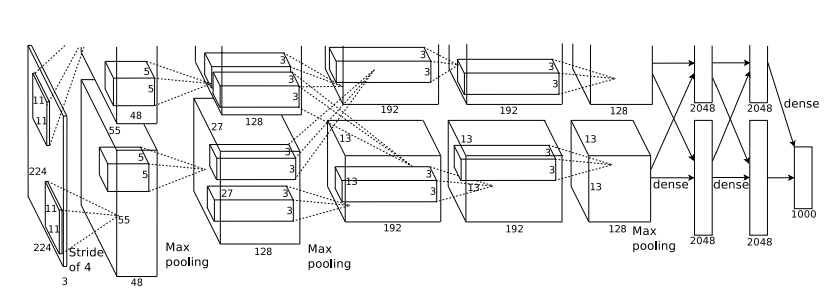
\includegraphics[width=0.8\textwidth]{img/AlexNet.png}
            \caption{Arquitectura de la red AlexNet. Destaca que parece estar \entrecomillado{partida} en dos mitades, esto es porque por primera vez se usaron las GPUs para entrenar la red de manera que una GPU realizaba la parte superior de la arquitectura y otra la parte inferior. Imagen extraida de \cite{krizhevsky2012imagenet}.}
            \label{fig:AlexNet}
        \end{figure}

        \noindent Destacan las siguientes propiedades:

        \begin{itemize}
            \item Tiene un total de ocho capas sin contar las de pooling, cinco convolucionales y tres FC.
            \item Emplea ReLU como función de activación en lugar de tanh pues se demuestra que acelera el proceso de entrenamiento $\times 6$ y obtiene un error del $25\%$ en el dataset CIFAR-10.
            \item Se emplearon múltiples GPUs para el entrenamiento dividiendo las neuronas en dos conjuntos. Esto aceleró aún más el entrenamiento.
            \item Emplean la técnica de Max Pooling en lugar de la de Average Pooling de LeNet. 
            \item Tienen 60 millones de parámetros que aprender, de manera que para evitar el Overfitting se usó la técnica de \textbf{dropout}, que consistía en \entrecomillado{apagar} neuronas en cada iteración del entrenamiento de acuerdo a una probabilida del $50\%$. También se usó \textbf{data augmentation} que explicaremos en \autoref{sub:data_augmentation}.
            \item El modelo ganó la competición ImageNet en $2012$ con una diferencia en precisión del $11\%$ con respecto al algoritmo que quedó en segundo lugar.
        \end{itemize}
    
    \subsubsection{GoogLeNet}
        \noindent La arquitectura de GoogLeNet está basada en un módulo que se denomina \textbf{Inception} creado con la intención de reducir el coste computacional de las CNNs. Para ello se propone que en vez de construir una red muy profundas se realicen simultáneamente múltiples convoluciones en una sola capa. Con este modelo aparecen los primeros filtros de convolución $1\times 1$ encargados de reducir la profundidad del volumen de entrada manteniendo las dimensiones.

        \medskip

        \noindent Con este modelo, se permitía realizar simultáneamente diversas operaciones sobre un volumen de entrada y finalmente se concatenaban los mapas de activación.

        \begin{figure}[!h]
            \centering
            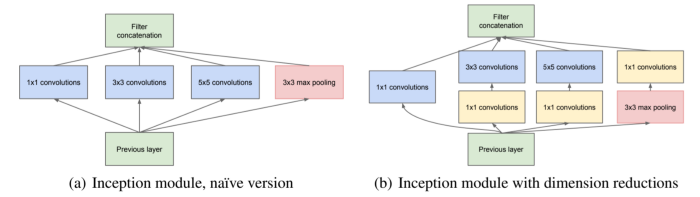
\includegraphics[width=0.8\textwidth]{img/inception_module.png}
            \caption{Ejemplos de módulos Inception.}
            \label{fig:inception}
        \end{figure}

        \noindent Con este nuevo módulo se desarrolló en 2015 la red GoogLeNet \cite{szegedy2015going}, que consiguió ganar el concurso ImageNet con empate técnico con la red \textbf{VGG-19}. En vez de usar capas FC usaron la técnica de \textbf{golbal average pooling} mediante la cual reducían la dimensión de los tensores con convoluciones $1 \times 1$.

        \begin{figure}[!h]
            \centering
            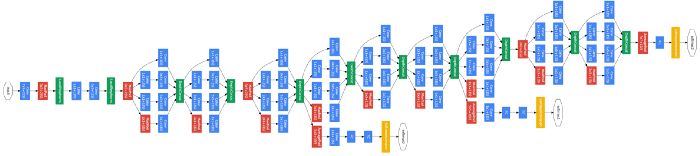
\includegraphics[width=0.8\textwidth]{img/GoogLeNet.png}
            \caption{Arquitectura de GoogLeNet usando módulos Inception.}
            \label{fig:GoogLeNet}
        \end{figure}

        \noindent Destacan las siguientes propiedades:

        \begin{itemize}
            \item Tiene un total de 27 capas de profundidad, por lo que aumenta notablemente la profundidad con respecto a sus antecesores.
            \item El uso de convoluciones $1\times 1$ con 128 filtros ayudan a reducir la dimensionalidad en lugar de usar capas FC.
            \item Contiene una capa FC con 1024 unidades y que alimenta una ReLU. 
            \item Tiene una capa lineal con Softmax para clasificación multiclase.
        \end{itemize}

    \subsubsection{VGG-16}
        \noindent Supuso un gran salto en rendimiento con respecto a los modelos anteriores. Los principales cambios con modelos anteriores como AlexNet es que dejaron de usar filtros de grandes dimensiones en las primeras etapas de la red para pasar a usar solo filtros $3 \times 3$. Esto ahorraba costes y permitía hacer una red más profunda \cite{simonyan2014very}.

        \begin{figure}[!h]
            \centering
            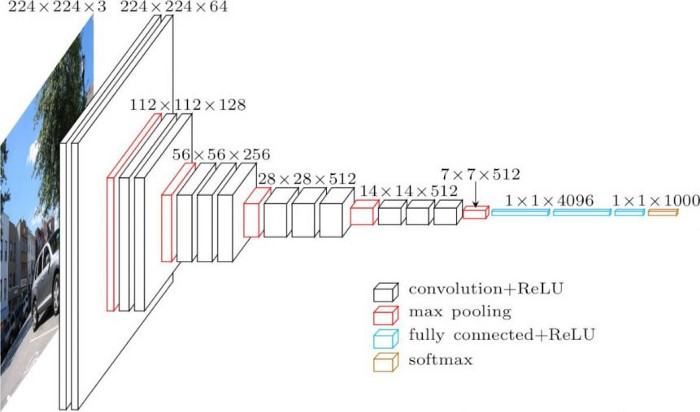
\includegraphics[width=0.8\textwidth]{img/VGG-16.jpeg}
            \caption{Arquitectura de VGG-16.}
            \label{fig:VGG}
        \end{figure}

        \noindent Destacan las siguientes propiedades:

        \begin{itemize}
            \item Consigue en Imagenet una precisión del $92.7 \%$.
            \item Tiene unos 138 millones de parámetros entrenables que es más del doble de cualquiera de los modelos anteriores, lo que hace que VGG-16 sea muy lenta de entrenar.
        \end{itemize}

    \subsubsection{ResNet}

        \noindent Tras los modelos anteriores, todavía quedaba un problema que tenían las CNN sin resolver, y es que cuanto más profundas eran, más problema había con el cálculo de los gradientes, pues tendían a cantidades infinitesimalmente pequeñas. Es por ello que surge la arquitectura \textbf{ResNet} \cite{he2016deep}, que introduce cortes en la red conectando un tensor con el que había unas cuantas etapas atrás, a esto se le denomina \textbf{bloque residual}. 

        \begin{figure}[!h]
            \centering
            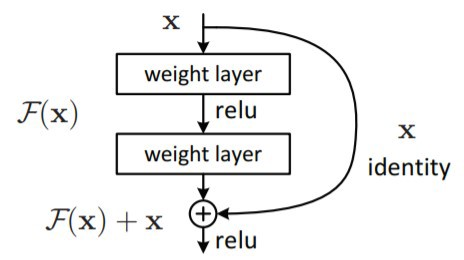
\includegraphics[width=0.5\textwidth]{img/resnet_module.jpeg}
            \caption{Bloque residual de una ResNet. Como vemos, se suma el tensor $x$ con el tensor $\mathcal{F}(x)$ que surge unas etapas después. Imagen extraida de \cite{he2016deep}.}
            \label{fig:Resnet}
        \end{figure}
        
        \noindent Con estos bloques residuales impedimos que los gradientes tiendan a cero rápidamente, con lo que podemos crear redes mucho más profundas. De hecho la versión de ResNet con 152 capas ganó el concurso ILSVRC 2015 siendo la red más profunda en aquel entonces. 

        \begin{figure}[!h]
            \centering
            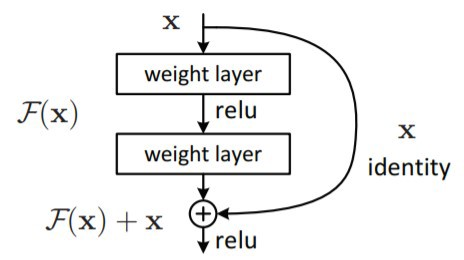
\includegraphics[width=0.5\textwidth]{img/resnet_module.jpeg}
            \caption{Resumen de los ganadores del concurso ILSVRC hasta 2015 con la aparición de Resnet. Imagen extraida de \cite{StanfordCourse}.}
            \label{fig:ImageNet}
        \end{figure}


\section{Autoencoders}
    \noindent Hasta ahora hemos visto qué son las CNN y su gran importancia en Deep learning en tareas de reconocimiento de objetos en imágenes. A continuación vamos a presentar un tipo de red que se emplea en tareas de \textit{Aprendizaje no supervisado} y que será de gran importancia en nuestro trabajo. Se tratan de las redes conocidas como \textbf{Autoencoders}.

    \subsection{Introducción}
        \noindent Los \textbf{Autoencoders} \cite{GAN2} son un tipo específico de red cuya entrada \entrecomillado{coincide} con su salida. Se encargan de reducir las imágenes de entrada a un vector perteneciente a un espacio vectorial latente y que idealmente codifica los elementos más relevantes en la imagen para posteriormente reconstruir la imagen a partir de este vector con la intención de que sea lo más parecida posible a la de entrada.

        \medskip

        \noindent Los autoencoders tienen tres componentes principales: 

        \begin{itemize}
            \item \textbf{Encoder}: Suele ser una subred que se encarga de codificar la entrada a un vector de un espacio vectorial latente. 
            \item \textbf{Code}: es el vector que codifica la imagen de entrada. 
            \item \textbf{Decoder}: se trata de una subred que reconstruye la imagen a partir del vector.
        \end{itemize}

        \noindent Como podemos ver, no se necesita ningún tipo de etiqueta para reconstruir las imágenes de entrada, por lo que este tipo de redes se emplean en tareas de \textit{Aprendizaje no supervisado}.

        \begin{figure}[!h]
            \centering
            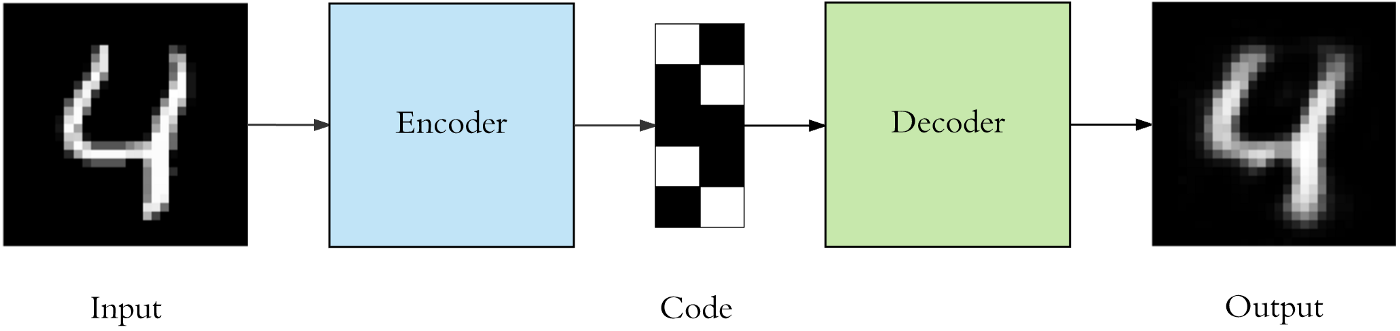
\includegraphics[width=0.5\textwidth]{img/Autoencoder.png}
            \caption{Esquema de un Autoencoder básico. Imagen extraida de \cite{GAN2}.}
            \label{fig:Autoencoder}
        \end{figure}

        \medskip 

        \noindent Esta estructura ha ido evolucionando durante los últimos años, por lo que vamos a ver a continuación esta evolución hasta llegar a la red que emplearemos en nuestro trabajo, el \textbf{Adversarial Autoencoder}.

    \subsection{Evolución de los Autoencoders}
        \subsubsection{Generative Adversarial Networks (GANs)}
            \noindent Es una red cuyo fin es \entrecomillado{crear nuevo contenido} y que sea lo más similar posible al contenido de la base de datos que usamos para entrenar la red. Para ello se pretende aprender la distribución de probabilidad que siguen los píxeles de las imágenes del dataset, por lo que el objetivo realmente sería el re generar nuevos valores aleatorios de la distribución de probabilidad que siguen las imágenes \cite{GAN}. 

            \medskip

            \noindent Para esta tarea suele emplearse una CNN denominada \textit{Generative Network} que tiene como objetivo recibir una imagen o un vector aleatorio y producir como salida una imagen de las mismas dimensiones que la de entrada que siga la distribución de probabilidad de las imágenes del dataset. Esta red tiene la estructura de un \textbf{Autoencoder}.

            \begin{figure}[!h]
                \centering
                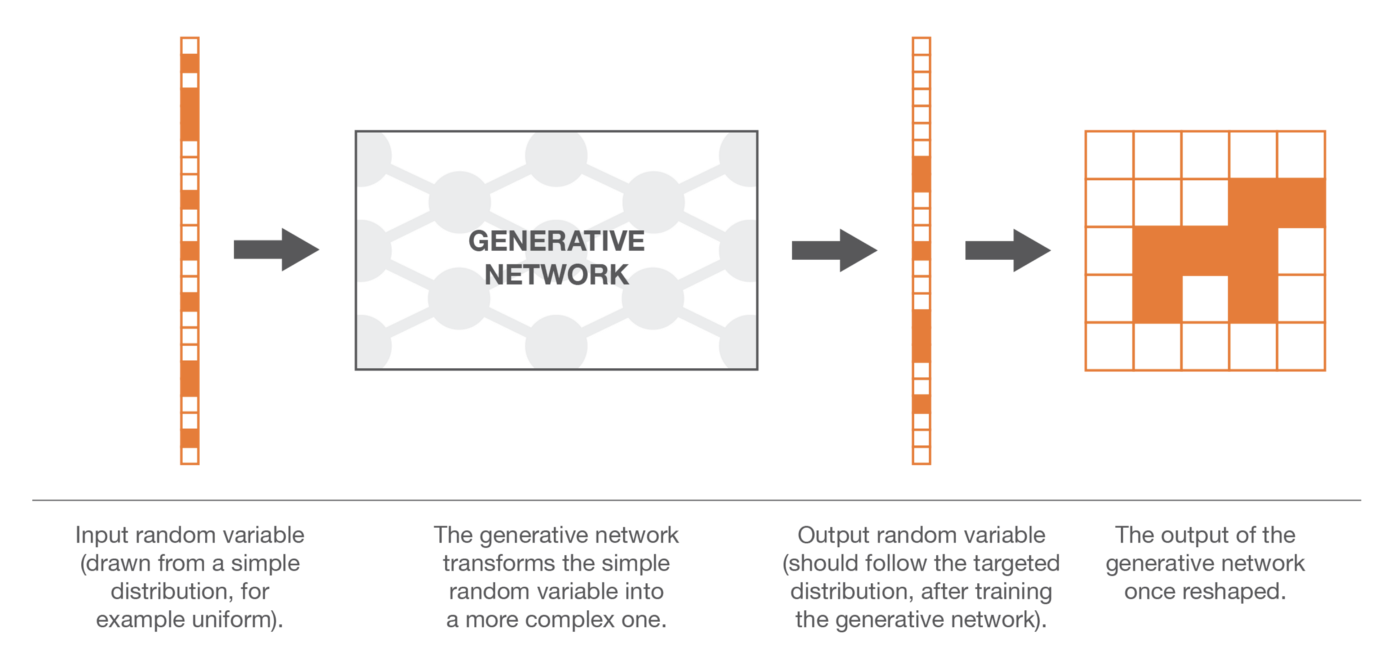
\includegraphics[width=0.5\textwidth]{img/Generative_network.png}
                \caption{Ejemplo de una Generative Network que pretende aprender la distribución de probabilidad de un conjunto de imágenes de perros. Imagen extraida de \cite{autoencoders2017}.}
                \label{fig:Generative Network}
            \end{figure}
            
            \medskip

            \noindent Por otro lado, se hace uso de una segunda CNN denominada \textit{Discriminador}, que recibe un conjunto de imágenes del dataset e imágenes generadas por el \textit{Genenerative Network} imagen de entrada y trata de clasificarlas en imágenes procedentes del dataset o imágenes generadas por la red. Por lo que el objetivo de la GAN en general podría resumirse en generar imágenes con la \textit{Genenerative Network} que sean capaces de engañar al \textit{Discriminador}, y para esto se pretende aprender lo mejor posible la distribución de probabilidad de las imágenes del dataset.

            \begin{figure}[!h]
                \centering
                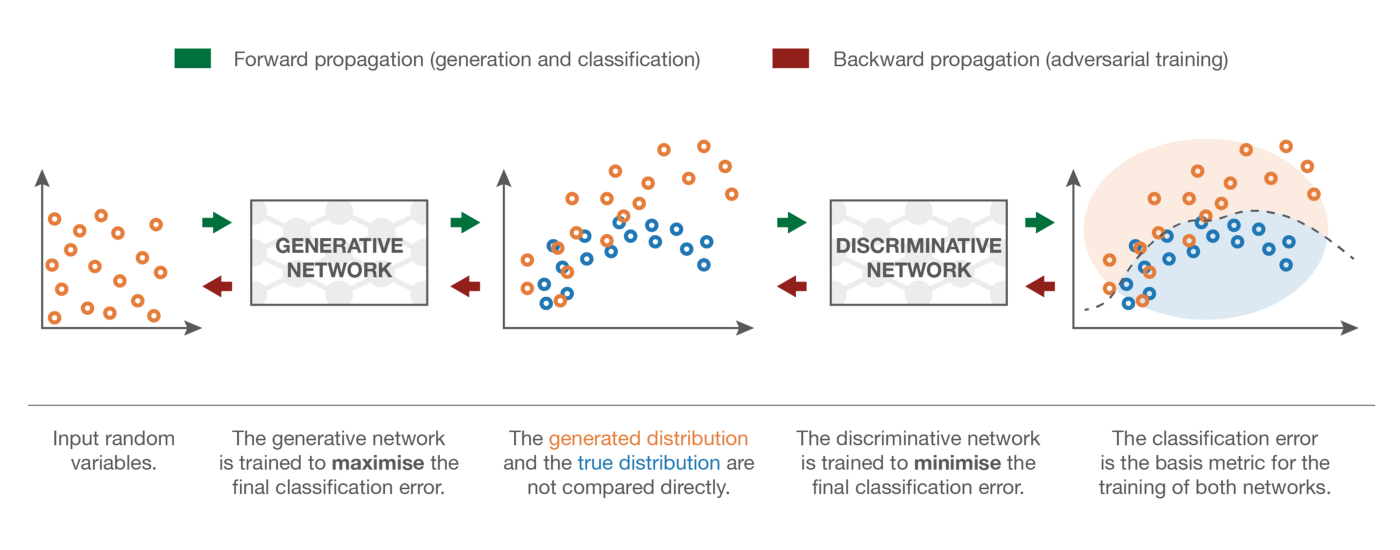
\includegraphics[width=0.8\textwidth]{img/proceso_entrenamiento_GAN.png}
                \caption{Resumen del proceso de entrenamiento de una GAN. Imagen extraida de \cite{autoencoders2017}.}
                \label{fig:Generative Network}
            \end{figure}

            \begin{figure}[!h]
                \centering
                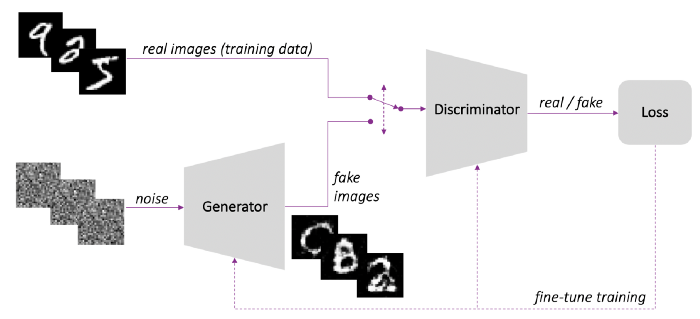
\includegraphics[width=0.5\textwidth]{img/GAN.png}
                \caption{Ejemplo de la arquitectura de una GAN para generar imágenes de dígitos manuscritos.}
                \label{fig:GAN}
            \end{figure}
 
        \subsubsection{Variational Autoencoder}

\section{Tratamiento de imágenes 2D y técnicas empleadas}
    \subsection{Tratamiento de imágenes 2D}

    \subsection{Data Augmentation} \label{sub:data_augmentation}

    \subsection{few-shot Learning}

\endinput
%------------------------------------------------------------------------------------
% FIN DEL CAPÍTULO. 
%------------------------------------------------------------------------------------

